% This file can be used to compile the adventure into a stand alone PDF without the sourcebook
\documentclass{book}


\usepackage{../../static/templates/fate_latex_template/fate_solarpunk}
\usepackage{montserrat}
\usepackage{ebgaramond}
\usepackage{hyperref}

%%%%%% Fixing overful hboxes
%% https://tex.stackexchange.com/questions/35/what-does-overfull-hbox-mean-why-is-there-a-black-mark-at-the-end-of-a-line
\usepackage{hyphenat}
%% \hyp{} can mark where words can break
%% Make it simpler:
%% https://tex.stackexchange.com/questions/488008/how-to-create-an-alternative-to-shortcut-or-hyp
\usepackage[english]{babel}


% Create title and background image
% https://tex.stackexchange.com/questions/136900/insert-a-full-page-image
% https://www.ctan.org/pkg/background
\usepackage[pages=some]{background}
\backgroundsetup{
scale=1,
angle=0,
opacity=1,
firstpage=true,
contents={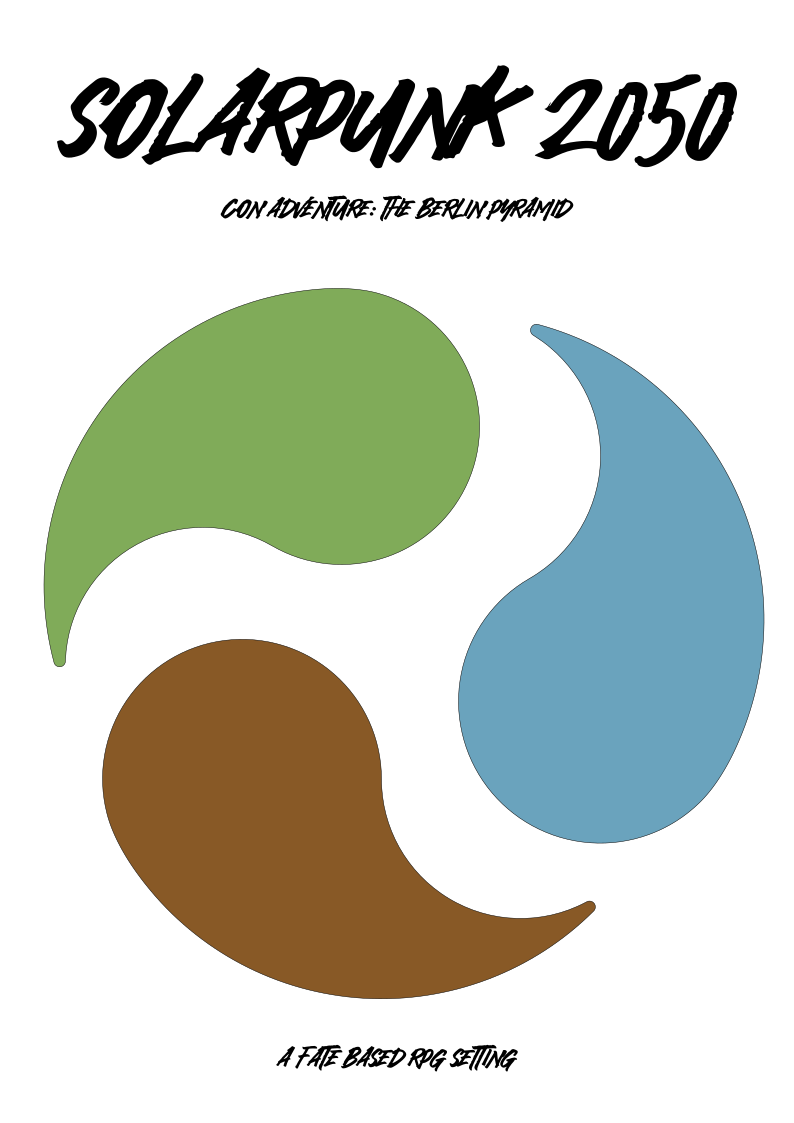
\includegraphics[width=\paperwidth,height=\paperheight]{../sourcebook/static/the_berlin_pyramid.png}}
}

\useshorthands{~}
\defineshorthand{~-}{\hyp{}}
%% ~- can mark this break now



%... other code

% \section{Hello World}
% \label{sec:hello}



% For creating example text
% \usepackage{lipsum}

\title{Fate Solarpunk 2050 - Adventure "The Berlin Pyramid"}
\author{Thorsten Sick}

\pagenumbering{arabic}
\begin{document}
%
% Book front page
%
\mbox{}
\thispagestyle{empty}
\BgThispage

%% Hyphenation database:
\hyphenation{meal-worm Mc-Gyver fa-mous be-cause}
%%%%%

\chapter{Introduction}

Solarpunk is a utopian science fiction genre. \textbf{Solarpunk 2050} is the setting in which this goal has almost been achieved. The protagonists, called Pioneers, live in ecological, technologically advanced and socially progressive communities. Close to the big cities, where the so-called Norms go about their daily lives - pampered by their AI.

This adventure is part of the Solarpunk 2050 setting, but contains everything you need to get started. It is based on Fate Condensed.

\section{Use cases}

This adventure is a con adventure. It can be played with new players and will take about 4 hours. The setting starts in the wide world but the characters will spend most of the time in a confined space. But it also perfectly fits into the mysteries of the first campaign in the core rulebook. If one of your players is missing and you still want to play, hand out these first pre-generated characters and play it. It will add a new facet to the events in the campaign.

\section{Test players}

Thanks you, test players at the CCC camp 2023 and new years eve 2023-2024. Your input made it into the final version.

\chapter{Project lifeguard}
\label{ch:project lifeguard}

\section{Topic}

Goal is to build a new community (or several ones: one for each faction), stop the evil plans of an old company (which is a relic) and give people new hope.

The protagonists can be from any faction. A mixed group is best.

The start of the adventure is well planned to get everything running smoothly. The core of the adventure (Albstadt) is a sandbox with characters, trouble and locations.

Here the players can start helping the people, building a community, fight the relic and find new friends. They cooperate - up until they will have to decide which type of community they are about to build:

\begin{itemize}
    \item Pioneer style
    \item Norm style
    \item Lost style
\end{itemize}

Their behaviour towards the NPCs and the style of their solutions to the problems will topple the NPCs towards one faction's philosophy or the others. The GM should take note and adjust the behaviour of the played NPCs.

In addition the NPCs can uncover some aspects of the main antagonists or the environment that can be used in the showdown.

The towns are based on real existing 2023 towns. For more details use Wikipedia and search for images.

This is full sandbox and I expect the players will create a new and unique community with its own traditions.

\section{Summary}

There is a town (Albstadt from the Swabian Alps, Germany) which got lost during the Dirty Road to Eden. The current inhabitants improvise to survive but never called for help. About 10 years ago they got contacted by the "Project Lifeguard" which sends them survival items. Most of that is quite cheap and even breaks their own small projects to become independent (like: cheap food kills local farming projects). After 10 years some people vanished. Others assume this could be connected to the Project Lifeguard and finally travel outside of their settlement to a Norm town. Short investigation: This Project is unknown and does not exist.

Truth is: Behind this project is an old company that is using a cave system in Albstadt to dump toxic waste. The Project Lifeguard is just a cover story and a cheap way to control the locals by making them dependent on continuous deliveries.

The Protagonists will be hired by the UN to investigate. They have a chance to help the locals, build communities or city hives in their fashion and uncover the evil plans of the \hyperref[sec: Relic]{relic}.

\begin{sidebarBox}[title=Relics]
\hyperref[sec: Relic]{Relics} are objects or organisations from the past. They do not fit into the new world and will be dismantled soon. The to dismantle list for those relics is long. And some just soldier on until it is their turn. Or they fight back.
\end{sidebarBox}

\begin{sidebarBox}[title=UN]
The \hyperref[sec: UN]{UN} is the last big institution left in 2050. It organised the global rescue efforts and introduced the Resource Point system. They are the good guys.
But it is also a kind of "franchise". Decentralized small organisations are a key for local action. This is where player characters can get their jobs from !
It can pack a punch if a big effort is needed, but will not act without proof and a dire situation.
Local action is preferred.

The UN has some camps with heavy machines including VTOL (Vertical Take off and Landing) and style helicopters. They use it to rescue people in disasters. And can be called only after a detailed investigation by people on the ground - the exact type of the disaster and the local situation has to be known first. The next camp is in Stuttgart.
\end{sidebarBox}

\section{Getting started}

The protagonists can earn \hyperref[sec:Resource Points]{Resource Points} if they help the UN to investigate the Project Lifeguard and help the people of Albstadt by building a Lost family, a Pioneer community or a Norm city hive (or all three of them) to integrate them back into civilisation.

First meeting is in the closest Norm town, the Sigmaringen Hive. Here all of them can meet the person who fled Albstadt and got picked up by the Lost.

\subsection{Scene one: UN meeting}

The player characters from all factions where called to the Norm town Sigmaringen for a UN meeting. Yet no one knows why. But they know: payment for helping the UN is Resource Points.

Norms use their AR interface called "\hyperref[sec:Hive controller]{Hive controller}" to organize projects, chat, meet online.... For the non-Norms people on the street seem to gesticulate with arcane hand movements interacting with something no Lost or Pioneer can see - they have no Hive controller.

They arrive independently (maybe at the train station or the zeppelin station next to it) and will meet the Norm characters at this location. Lost characters from their camp close to Albstadt could also simply have walked there. Lost and Pioneers will not know how life in a Norm Hive really works. Even if they life close by.
Non-Norm guests will receive a Hive controller as a gift. These devices are not yet configured and the new users did not do any tutorials. The usability of those devices is limited to what a 2 year old Norm could get out of his first device. But at least the controllers contain some Euro for expenses store to pay for premium services during the trip to the UN meeting.

Sigmaringen is a nice and relaxed town. Many roads have been replaced by parks after 2020. Tame deer are walking around and can be fed (or they steal anything that looks like food). Solar panels are attached to every available surface. Public transport is working flawless and is based on amphibious buses to also use the Danube. In the town and in the public vehicles there are shelves where people can get free food and other things of basic need. This is normal for the Norms and may seem strange for Lost and Pioneers.

Next to the train station is a large zeppelin airport with several logistics companies using those airships to transport standard containers.

Sigmaringen is self sustaining with a large \hyperref[sec: norm food]{Ceres} food production centre.

On a small hill in the centre of Sigmaringen is a castle. Solar panels were added to it during the last years - but their integration is so well done they are hard to notice. It is in 5 minute walking distance from the train station. Walking there the non-Norms can experience a modern city, free public transport, free food vending machines, deer, trees and a small brook cris-crosing the city streets.

The meeting room in the castle was prepared for the UN conference. Someone got the "Emergency UN meeting props box" from the attic and decorated everything with large and small flags, placed cards on the table with UN logo, installed a UN logo on the big video screen in the room.

After all the characters arrived they are greeted by city officials who also do not know why everyone is here (but are proud to host a UN conference).

Perfect last chance for the characters to introduce each other before the UN meeting starts.

After a short time a UN official appears on the screen (from Addis Ababa, Ethiopia). Her name is Enku and she is experts for relics.
The connection to Africa is run over some glass fibre tracks, some high flying repeater drones and other network hacks. Satellites do not exist any more after the \hyperref[sec: Kessler Syndrome]{Kessler Syndrome}.

The characters receive a mission:
The next town "Albstadt" is a no-go area and a relic. It was destroyed when the caves under the area caved in. Caused by low water levels over several years. A Lost family camped close by (the family of the characters in the meeting). Something strange happened there. But the characters can tell the story themselves.


\subsection{Flashback for Lost: T minus 5}

Takeaways:

\begin{itemize}
    \item Kim fled from Albstadt. It is still inhabited !Finding refugee at the Lost camp. Badly injured and unconscious.
    \item A professional fighter chased this person - obviously equipped with illegal Cyberware (which means: replacement parts enhanced normal human abilities)
    \item Kim claimed the project "Lifeguard" supports the town. But life there is harsh. Before losing consciousness.
\end{itemize}


The lost camp is in between Sigmaringen and Albstadt in the wilderness. Close to Winterlingen. Albstadt and Sigmaringen are part of the Lost hunting ground. But they respect the Norms in Sigmaringen and will not be caught hunting the deer there. And they know that the No-go area around Albstadt is high-risk and avoid that region. The camp is mobile and consists of diesel vehicles and tents. No Lost knows what happened in Albstadt 20 years ago. No one is allowed to go there. But they raid the outer ruins for stuff.

At the evening, while partying eating "Risotto Rodenti" (containing rats, squirrels and especially invasive species) and playing \hyperref[sec:Shakespeare battle]{Shakespeare battle}.

While they partying the Lost guards at the perimeter stop a person fleeing from Albstadt. The person wears rags. A military grade Cyborg hunts this person.

The guards at the perimeter stop the Cyborg by gunfire. As soon as the Cyborg loses the battle the Cyberware self destructs and kills him. The Cyberware is obviously illegal.

(The player characters are not part of the fight. But they can assist later: First aid, investigate the cyborg, ... This is why they know the essential info first hand).

The rescued person (named Kim) tells a strange story:

He was born in Albstadt. Which is almost 100 percent destroyed. The caved in area made the whole town very vertical. Some ruins of buildings are still attached to rocky spikes. Caves are accessible now where no caves have been before. The people build makeshift bridges and were waiting for help. 10 years ago it arrived. \textbf{Project Lifeguard} came. The Cyborg belongs to this project.

They visit once a month and bring the bare minimum. Food, medicine, water, power (a fuel cell in a cargo container and enough hydrogen for a month). The town is fully dependent on them (which is the plan of project Lifeguard).

People started to disappear. This is why Kim fled. Kim soon loses consciousness and needs professional medical attention. This can be found in Sigmaringen.

Kim will be brought to a hospital in Sigmaringen. As soon as he gains consciousness he will be questioned and can be witness in the UN meeting later via video call.

\subsection{Flashback for Norms: T minus 3}

The Norm people in the room got the UN task to investigate a few days ago. Right after Kim was brought to the hospital and the incident was reported. The only clue they got was "What is Project Lifeguard ? They do ship 3 containers per month containing survival gear."

Their investigation can happened in AR mode only while the characters were enjoying their free Latte Macchiato with Soy milk and cakes somewhere at a Danube beach in Sigmaringen. Or they can do some breaking and entering at the shipping terminal. Or con the people working there.

Other options: phoning people, going through online databases, checking web cams and controlling drones.

They can learn:

\begin{itemize}
    \item The containers with the project logo are from Sigmaringen
    \item The Project Lifeguard is not registered anywhere !
    \item So officially those containers never start there
    \item A company called "Dumpit waste management incorporate" has the same ware house and is a daughter company of "Cargo !" which does all kind of shipping using Zeppelins
    \item The 4 "Dumpit" containers are shipped by Zeppelins drones to Albstadt
    \item Only one is paid for by the institutions wanting send the waste to recycling
    \item Dumpit is the only company shipping container this same way - passing Albstadt and sending them to a recycling plant in Luxemburg (this is the official version. In reality they just dump the waste in Albstadt. This is not revealed yet)
\end{itemize}

Entering the "Cargo !" container area they will learn that the container all look the same with a printed on ID code. The logo on the containers can be changed within seconds because it is just a giant multi-color e-paper. This is also why no container with the logo "Project Lifeguard" can be found there but literally appears in mid air.

A cargo Zeppelin can carry 4 containers and can lower them with a crane. A default run to Luxemburg is 1 Dumpit waste container and 3 Project Lifeguard containers. They all start with the Dumpit logo.

\subsubsection{Zeppelin pilot Luke}

Luke is the Zeppelin pilot for "Cargo !". He has the strong suspicion that something is wrong with the Dumpit job. But he also knows: investigating and digging deeper will just confirm it and then he will have to decide if he wants to keep a good job or not. When approached on a personal level a very good \textbf{Rapport} job could get some information out of him:

\begin{itemize}
    \item He never flies to Luxemburg
    \item There is a stop in Albstadt
    \item It is not a wasteland as expected. But he will not tell more
    \item He starts with 4 Dumpit containers (not mentioning 3 will be rebranded mid-flight)
    \item He never mentions what happens to those containers in Albstadt. Not the 3 dropped at the Supermarket, not the one emptied into the "bottomless sinkhole"
\end{itemize}

Some of those topics make him feel uncomfortable. He will evade talking about his favourite show he watches while flying his delivery tours.


\subsection{Flashback for Pioneers: T minus 2}

The Pioneer camp is at the former university campus on a hill close to Sigmaringen. The Pioneers occupied the deserted university campus 10 years ago (the climate catastrophe made everyone flee this location). The boring cement buildings are exactly as they were, except:

\begin{itemize}
    \item The interior is now decorated with unicorns or strange experiments are in the hallways
    \item On the outside and between the buildings a high-tech shanty town has been erected. From human sized honeycombs glued to a wall for accommodation to a small robot tended garden
    \item The laboratories are used but not abused. This is the wealth the Pioneers found there
\end{itemize}

This university campus is 30 minutes walking distance from Sigmaringen (for the Lost). 5 Minutes taking an experimental Pioneer electric trike with AI assisted dampers - risk level low. Or just call a public transport and drive 15 minutes and have a coffee and croissant (Norms).
The Pioneers think Sigmaringen is boring and normally don't visit it.

The mission: The UN needs a scout robot with building capability in this region. Fast. The Pioneer community advertised their robot some time ago and this is why they get a call to send their robot and 1-2 operators for it.

The UN call gets everyone hyped. So the community decides to do a party and some last-minute fixes and improvements ....

Those fixes are all introduced by mildly intoxicated crazy engineers (Pioneers....) and harvest parts from other projects. The player characters can defend the current features of the robot or push on. For every fix a "Prototyping" roll is made and the robot gains the listed features, on a failed dice throw it will also get a new glitch. See the list below for ideas.

The robot starts as a semi-autonomous building bot. The bot is table sized, has 6 legs, a nozzle to distribute a self hardening concrete for building and can run with battery and concrete storage of 6 bucket sized containers. It is remote controlled.

Modifications, suggested by the party people:

\begin{itemize}
    \item Gecko grip (on fail: will accidental stick to people and other objects)
    \item Waterproof, 10 meters (on fail: building gets flooded during test run)
    \item Other material: wood pulp, plastic (on fail: ugly test object sticks to the floor an no one knows how to remove it)
    \item Can process wood into wood pulp (on fail: people kept feeding it furniture in their enthusiasm)
    \item Feed pipe for large scale projects (on fail: The community is now in possession of a large scale video character monument....)
    \item Autonomous option (on fail: starts printing strange objects when no one is looking)
    \item Colour cartridge (on fail: can only print rainbow coloured things now)
\end{itemize}

Finally the Pioneer kids will paint it with shiny colours beetle style and add goggly eyes. This is not optional.

After that the delegation leaves for Sigmaringen, with the robot to meet the other groups at the UN meeting.

\subsection{UN meeting continued}

After that the UN meeting can continue. Kim can be questioned, the protagonists get the offer to receive Resource Points in exchange for their help, .... and are sent towards Albstadt. Maybe with a short stop at the Lost camp in between.

Some players will want to start investigating in Sigmaringen - now that the basic problem is known. Encourage them. They can find many answers. But not enough to satisfy the UN. They will want some on site investigation to confirm the suspicions.

\section{Areas}

\subsection{Sigmaringen Hive}

Sigmaringen is already described in the UN meeting section.

The protagonists can start investigating in Sigmaringen. Here they can find a mesh of companies and shell companies all belonging to "Cargo !".

\subsection{Lost camp}

If the players want to visit the Lost camp in between Albstadt and Sigmaringen they will find:

\begin{itemize}
    \item Several diesel trucks
    \item Tents
    \item A whiteboard with a sector map (Including Sigmaringen and Albstadt. With Sigmaringen marked with "Food" + "inhabited" and Albstadt marked as "no-go" + "danger")
    \item A kitchen ready to cook rabbit stew and the deer a team of hunters caught "close to Sigmaringen". The kitchen has camping level hygiene standards. And eating real animals can confuse Norms.
    \item A library in a protected old school bus. Visitors can read books but are not allowed to touch them.
    \item The Hive controllers will already start to lose radio connection to the Hive. This will make the Norm characters very nervous.
\end{itemize}

The sector map is a map a Lost group will start to build as soon as they arrived somewhere. The area is split into sectors with the camp in the centre. Teams start to investigate what they can find in each sector: food sources, ruins, threats, ... Interesting is in this case: the area around Albstadt marked as "threat, do not access". On the other side is Sigmaringen, marked as "food source (deer)".

When entering the camp with a Lost guide this guide will have to pledge for his friends. On doing that the visitors are searched for weapons. If none are found they will \hyperref[sec:Lost guests and weapons]{receive easy to use guns}.

\subsection{Forest: The no-go area close to Albstadt}

There is a fence with lots of warning signs close to Albstadt. The area looks like a normal forest. But looking closely you can see 50m deep ditches starting short after the fence. Closer to Albstadt those ditches can be up to 200m deep. So the danger is real.

The trick to crossing it is to build a kind of bridge to support the brittle forest floor. With the Pioneer robot this is a piece of cake. But wooden boards and some testing the ground can help as well.


\subsubsection{Action scene}

Halfway to Albstadt some wild boars will act as agents of chaos to create a life threatening situation. The boars are not attacking directly. But flushed out by the visitors they act unwise and trigger the real threat: Falling trees (falling to the side or vertically vanishing into a new 50m ditch), breaking forest floor, ...
the whole landscape becomes the enemy and fighting the boars (to reduce the amount of chaos) or tinkering to build some stable ground or secure the remaining trees will be needed to safe the day.

\subsubsection{Part of the solution}

The forest can be part of the solution should the protagonists want to create a self sufficient Albstadt. There is fertile soil for farming and tasty animals. The stability is an issue. But with good mapping and some structural fixes parts of the forest can be accessible.

\subsection{Albstadt}

From the edge of the forest the protagonists can see a deep slope (about 200m deep) and on the ground flowing water. The remains of Albstadt are on spires reaching out to normal ground level.

Albstadt was destroyed in a disaster. The karst area caved in. The landscape is more vertical with cliffs than horizontal now. Some buildings have been structurally secured to prevent them from falling completely into the ditches. There are improvised bridges everywhere. Caves have opened. Some are filled with water and need diving gear to reach the ground (where maybe some valuables from the disaster ended up).
The people here did a good job at surviving in their broken town. But they did not dare to reach out for help. They were found by Project Lifeguard but the help sent through that made them even more dependent.

(For the cave system: Check out "Blautopf" on Wikipedia)

\subsubsection{General}

Albstadt is a maze of spires, where the tops of the spires are at ground level. The canyon system is filled with water and caves (dry or filled with water) are everywhere.

Old buildings either survived at the top of the spires or are hanging at the side. With heavy damage and secured by ropes.

Between the spires there are improvised suspension bridges and supply lines to the supermarket (power, water). All of that needs repair or replacement.

At the beginning of the adventure the Sigmaringen hive will drop a radio repeater close to Albstadt. The Norms will have a connection to the Sigmaringen hive. No dice penalty but delivery time is +1h.

\subsubsection{Supermarket}

The supermarket is the largest surviving structure. It is controlled by Ash and his goons. Ash is the local despot. The parking space in front of the supermarket is where the containers are dropped by cargo zeppelins. Those are instantly secured by Ash and the goons.
They will store the goods in the supermarket (which is filled with shelves of wealth).

While the parking space and the main building of the supermarket look intact the whole backside wall of the building is missing. It fell down the side of the spire. From a security perspective this is not an issue because no one living there could climb up the spire wall and enter that way. Or build a bridge or stairs by using a robot - this is an option the protagonists have.

In the Supermarket there are lots of shelves with an epic amount of food and tools. A small but fancy set of rooms where Ash lives and Ash's office. Here he keeps all the dirty secrets he collected about Dumpit.

\subsubsection{Part of the solution}

\textbf{Problem:} It is controlled by Ash and his goons. He uses it to control the whole town by artificial scarcity
\textbf{Solutions:} Get rid of Ash, blackmail him
\textbf{Benefits:} A building for storage, crafting, town centre, ....

Ash also has lots of blackmail material to bring Project Lifeguard and Dumpit down.

\subsubsection{Leo's}

\textbf{Leo} tried to fix his building and spire as good as possible. But he was lacking material and technology. After killing a person by accident (throwing a stone to help Kim escape) he is in a depressed state. In his current mental state he can not help - but maybe someone can help him out of that. And get him some tools !

\subsubsection{Part of the solution}

\textbf{Problem:} Leo does not have the technology to properly build what he wants to build
\textbf{Solution:} Scale up, use Pioneer tech, order stuff from Sigmaringen
\textbf{Problem 2:} Leo is mentally unstable after accidental killing someone
\textbf{Solution 2:} Leo needs therapy (long term solution) or a call to action (and more therapy later)
\textbf{Benefits:} A first hanging garden, proper bridges and supply lines. A showcase for more improvements and a free Albstadt.

\subsubsection{Lara's}

\textbf{Lara} dwells in a old house with broken roof on a spire. Here she cares for three poisoned people. The only special thing about her spire is a long ladder reaching down to the small dock she built at the water level where she keeps here canoe.
In her home she cares for three ill people. They all went to the secret Dumpit cave downriver and brought back a "glows in the dark" lucky charm. A shard of radioactive material which was part of the waste dumped there. This shard caused radiation sickness. They still keep it around and Lara is not aware of the threat.
Lara is the person who knows the region. Especially the wilderness. If the patients are cared for (maybe with Norm/Pioneer tech) she can show people around. That way sources for water, food and renewable electricity can be found. Also places to prepare an ambush for the showdown.

\subsubsection{Part of the solution}

\textbf{Problem:} Lara has to care for the patients
\textbf{Solution:} Care for the patients with proper medical tech
\textbf{Benefits:} A proper map of the natural area with different sources for food, water and energy. And places for an ambush

\subsubsection{Water level maze}

This is where \textbf{Lara} spends her time: 200 m below the top of the spires. There are water ways with beaches, rapids, caves and large rocks in the water. Most of the water is drinkable (basic filtering is advised). The animals and plants can be eaten. Which the people living there do not know.

A small boat or canoes will be relevant for travelling.

There are a lot of dangerous caves. For natural reasons. Downriver there is one cave where the toxic waste was dumped. Staying there without protective equipment can be dangerous. Also: Do not eat the crabs there.

%% https://en.wikipedia.org/wiki/Orphan_source

\textbf{Problem:} American crabs are eating the local life
\textbf{Solutions:} Build traps, eat the crabs
\textbf{Benefits:} Food

\subsubsection{Sams bunker}

\textbf{Sam} (she/her) hides in a bunker like control structure. It is built to house 20 people it was the home of 3 until recently (the cyborg and Sams colleague got killed). With his colleagues being killed he is in shock. He is also not happy with the project he is in. He wanted to do something good but it turned out the project he signed for is a fraud and harming the people of Albstadt. The last few days he collected log data and notes covering what happened the last few years (he himself arrived a few months ago, but the logs go back for many years). This information can destroy Dumpit and all people involved.

\textbf{Problem:} Sam is scared and hiding there.
\textbf{Solutions:} Talk, produce some prove the situation calmed down
\textbf{Benefits:} Workshop, drones and information about Dumpit

% What is left ? Church as city assembly. An old super market as source for tools, a museum for local history (really old farm tools),
% People life in shanty town, makeshift tents
% How did the project replace essential things ? Power => Battery container, Food => Cans, Water => Bottles, Medicine => A doctor visits once a month
% Who is left ? Some people could build a sustainable life. Lifeguard is blocking that.
% How do they interact ? Some people love the dependency on PLG
% What can they find out ? Something is going on in the tunnels. The help is keeping people down.
% How can they rebuild ? Start gardening, build water cisterns,
% Who can be recruited & empowered ?
% How will PLG respond ? Sabotage and violence ? What before that ? Threats ?
% Supermarket owner gets gunned by PLG to defend the last resources
% Person who wants to do medic only gets basic material and everyone has to wait for the monthly visit of PLG for real help
% There is a spy for PLG, but this spy can be turned and used against PLG

\subsection{People at Albstadt}

In Albstadt there are about 200-300 people. Most of the people suffer from learned helplessness acquired in the last 30 years. They even forgot how to cook and just use the microwaves with the pre prepared meals offered by Project Lifeguard. With some very active ones struggling to keep everyone alive. But Project Life~-guard tricked them into non-sustainable ways to struggle and building more and more dependencies to Project Life~-guard. Those people could - using their skills smarter and more coordinated - build an in~-dependent Pioneer Community/~-Lost Family or Norm Hive. Until then they are a problem because they maintain the stupid structure tactically implemented by Project Lifeguard.

Those are the NPCs to interact with.

\section{NPCs}

\newpage

\begin{npcBox}[title=Leo]

    \begin{aspects}
    \item \aspect[High Concept]{An architect}
    \item \aspect[Trouble]{I will hulk out if you make me angry}
    \item \aspect[Aspect]{I dream to build big but the situation keeps me small}
    \end{aspects}

    \begin{skills}
        \item \nskill{Academics}{3}
        \item \nskill{Athletics}{1}
        \item \nskill{Burglary}{0}
        \item \nskill{Contacts}{1}
        \item \nskill{Crafts}{4}
        \item \nskill{Deceive}{0}
        \item \nskill{Drive}{0}
        \item \nskill{Empathy}{1}
        \item \nskill{Fight}{2}
        \item \nskill{Investigate}{0}
        \item \nskill{Lore}{1}
        \item \nskill{Notice}{0}
        \item \nskill{Physique}{3}
        \item \nskill{Provoke}{0}
        \item \nskill{Rapport}{0}
        \item \nskill{Resources}{2}
        \item \nskill{Shoot}{0}
        \item \nskill{Stealth}{0}
        \item \nskill{Will}{2}
     \end{skills}

    \begin{stunts}
    \item \stunt{Improvising}{Leo gets a +2 on Crafts when building architecture with alternative materials or scrap.}
    \end{stunts}



    \begin{stressSection}
    \stressLine{\stress{1}\stress{1}\stress{1}\stress{1}\stress{1}\stress{1}}{\stress{1}\stress{1}\stress{1}\stress{1}}
    \end{stressSection}
    \begin{tabularx}{\textwidth}{ XX }
    \end{tabularx}

    \begin{consequences}
    \item \consequence{2}
    \item \consequence{4}
    \item \consequence{6}
    \end{consequences}

    \begin{npcDescription}
    An impulsive architect, has a spire with a house on it. He tries to farm the side of the rock by attaching small boxes for plants.
    He was a part of the 5 minute rebellion where Kim fled. Being impulsive he threw rocks at the three people from project lifeguard. The Cyborg followed Kim. A rock thrown by Leo hit an engineer, throwing him of a bridge and killing him. Sam, the third engineer did hide in their bunker. Some antenna got destroyed by thrown rocks.
    After the rebellion turned bloody Leo withdrew. Shocked by his own action.
    If this gets fixed they can gain support by a skilled architect who just lacks the tools to build awesome vertical gardens and bridges.

    \textbf{Location:} His own spire. With a small house (repaired). And a small hanging garden at the side of the spire (just some flower pots, he did not have the right tools for proper hanging gardens)
    \textbf{Problem:} Has to deal with having killed someone. Maybe talking to Sam could help
    \textbf{When convinced:} Can help building stuff ( a real hanging garden, proper suspension bridges, traps for crabs)
    \end{npcDescription}

\end{npcBox}

\newpage

\begin{npcBox}[title=Lara]

    \begin{aspects}
    \item \aspect[High Concept]{One woman rescue operations}
    \item \aspect[Trouble]{Ready to sacrifice for others}
    \item \aspect[Aspect]{Knowledge of the country I spend my time with}
    \end{aspects}

    \begin{skills}
        \item \nskill{Academics}{0}
        \item \nskill{Athletics}{2}
        \item \nskill{Burglary}{1}
        \item \nskill{Contacts}{0}
        \item \nskill{Crafts}{0}
        \item \nskill{Deceive}{0}
        \item \nskill{Drive}{3}
        \item \nskill{Empathy}{0}
        \item \nskill{Fight}{2}
        \item \nskill{Investigate}{2}
        \item \nskill{Lore}{0}
        \item \nskill{Notice}{4}
        \item \nskill{Physique}{3}
        \item \nskill{Provoke}{0}
        \item \nskill{Rapport}{0}
        \item \nskill{Resources}{0}
        \item \nskill{Shoot}{1}
        \item \nskill{Stealth}{1}
        \item \nskill{Will}{1}
     \end{skills}

    \begin{stunts}
    \item \stunt{Just standing here}{Lara can get a +2 on Notice when silently observing people. As long as she can use a cover story involving her trips into nature or helping people.}
    \end{stunts}


    \begin{stressSection}
    \stressLine{\stress{1}\stress{1}\stress{1}\stress{1}\stress{1}\stress{1}}{\stress{1}\stress{1}\stress{1}\stress{1}}
    \end{stressSection}
    \begin{tabularx}{\textwidth}{ XX }
    \end{tabularx}

    \begin{consequences}
    \item \consequence{2}
    \item \consequence{4}
    \item \consequence{6}
    \end{consequences}

    \begin{npcDescription}
    Lara is a kind guide, knows all of Albstadt. She wants to uncover the truth about the cursed and haunted cave, the so called secret site, where the Project drops the poisonous garbage. It is not really haunted. But the people who went there soon died of disease.
    When doing this investigation the guide would have to abandon an important duty: care for people she rescued after accidents. They need medical care and leaving for 1-2 days is not an option.

    \textbf{Location:} At home (which needs repair) caring for the injured people. Some travelling.
    \textbf{Problem:} Needs someone to care for the injured people.
    \textbf{When convinced:} Can help exploring Albstadt and the haunted cave.
    \end{npcDescription}

\end{npcBox}

\newpage

\begin{npcBox}[title=Sam]

    \begin{aspects}
    \item \aspect[High Concept]{Scared good samaritan}
    \item \aspect[Trouble]{Are we the baddies ?}
    \item \aspect[Aspect]{Helper with evil masters}
    \end{aspects}

    \begin{skills}
        \item \nskill{Academics}{4}
        \item \nskill{Athletics}{1}
        \item \nskill{Burglary}{0}
        \item \nskill{Contacts}{0}
        \item \nskill{Crafts}{3}
        \item \nskill{Deceive}{0}
        \item \nskill{Drive}{1}
        \item \nskill{Empathy}{1}
        \item \nskill{Fight}{0}
        \item \nskill{Investigate}{0}
        \item \nskill{Lore}{1}
        \item \nskill{Notice}{2}
        \item \nskill{Physique}{0}
        \item \nskill{Provoke}{0}
        \item \nskill{Rapport}{3}
        \item \nskill{Resources}{2}
        \item \nskill{Shoot}{0}
        \item \nskill{Stealth}{0}
        \item \nskill{Will}{2}
     \end{skills}

    \begin{stunts}
    \item \stunt{I know my bunker}{Sam spent the last weeks studying the bunker and the computers there. Sam gets a +2 on Academics when asnwering bunker related questions.}
    \end{stunts}

    \begin{stressSection}
    \stressLine{\stress{1}\stress{1}\stress{1}}{\stress{1}\stress{1}\stress{1}\stress{1}}
    \end{stressSection}
    \begin{tabularx}{\textwidth}{ XX }
    \end{tabularx}

    \begin{consequences}
    \item \consequence{2}
    \item \consequence{4}
    \item \consequence{6}
    \end{consequences}

    \begin{npcDescription}
    Sam is the last of the three Project members. She wants to help people but is restricted by the company guidelines. Sam does not know anything about the poison dump (besides hints in the logs and some observations). At the beginning she was helpful but is now scared after the short escalation, the "revolution". As engineer and medic she could care for the injured people. If she would not be scared.

    Also: The antenna to the HQ is damaged. Sam not contact and ask for help.

    Keep in mind: There is some good in this NPC. But she works for the baddies.

    With some convincing she can become a powerful asset and friend. Helping with medicine and engineering. And also knowing (or guessing) some of the internals of Dumpit.

    \textbf{Location:} The company bunker. Or exploring the town via drones and getting into contact (the drones have speakers)
    \textbf{Problem:} Scared by the attack. Also doubts that the company is helping
    \textbf{When convinced:} Can offer medical help. Some engineering and insights into Project Lifeguard and the company "Dumpit"
    \end{npcDescription}

\end{npcBox}

\newpage

\begin{npcBox}[title=Ash]

    \begin{aspects}
    \item \aspect[High Concept]{Brute with power}
    \item \aspect[Trouble]{I am totally dependent on project Lifeguard}
    \item \aspect[Aspect]{Obey: I have the food, water and power}
    \item \aspect[Aspect]{A budget bond villain}
    \item \aspect[Aspect]{The art of running away in a smart way}
    \end{aspects}

    \begin{skills}
        \item \nskill{Academics}{0}
        \item \nskill{Athletics}{1}
        \item \nskill{Burglary}{1}
        \item \nskill{Contacts}{2}
        \item \nskill{Crafts}{0}
        \item \nskill{Deceive}{2}
        \item \nskill{Drive}{0}
        \item \nskill{Empathy}{0}
        \item \nskill{Fight}{3}
        \item \nskill{Investigate}{0}
        \item \nskill{Lore}{0}
        \item \nskill{Notice}{1}
        \item \nskill{Physique}{2}
        \item \nskill{Provoke}{3}
        \item \nskill{Rapport}{0}
        \item \nskill{Resources}{4}
        \item \nskill{Shoot}{2}
        \item \nskill{Stealth}{0}
        \item \nskill{Will}{1}
     \end{skills}

    \begin{stunts}
    \item \stunt{Prepared}{Can use Resources instead of Athletics when running away as long as Ash has prepared the escape route with gadgets to help escape}
    \item \stunt{Brave henchmen}{Ashs henchmen protect him and would even sacrifice their life (3 self sacrifices per story)}
    \item \stunt{Broken civilians}{Once per story Ash can get a +2 on Provoke to motivate broken civilians from Albstadt to help him - aginst their own self interest.}
    \end{stunts}


    \begin{stressSection}
    \stressLine{\stress{1}\stress{1}\stress{1}\stress{1}}{\stress{1}\stress{1}\stress{1}\stress{1}}
    \end{stressSection}
    \begin{tabularx}{\textwidth}{ XX }
    \end{tabularx}

    \begin{consequences}
    \item \consequence{2}
    \item \consequence{4}
    \item \consequence{6}
    \end{consequences}

    \begin{npcDescription}
    The old supermarket is the central hub for food, resources and power. Everything is delivered there. Ash, the owner of the supermarket got recruited to distribute it. The power soon corrupted him. He now controls the town. And thanks to blackmailing he can also control the Project Lifeguard deliveries.

    He already has some dirty secrets he uses to blackmail Dumpit. But to get even more power over his masters (the Project) he wants to investigate what is in the secret waste dump that poisons people.

    Ash is the real baddie

    \textbf{Location:} Supermarket
    \textbf{Problem:} Dependent on the Project Lifeguard. Wants to blackmail them. Just in case.
    \textbf{When convinced:} Can not be convinced. Just blackmailed, forced, .... will then offer control over the whole settlement and the data on Dumpit
    \end{npcDescription}

\end{npcBox}




\subsection{Project Lifeguard by Dumpit waste management inc.}

History:
\begin{enumerate}
    \item 30 years ago Albstadt was destroyed by the disaster
    \item People managed to survive
    \item 10 years ago Dumpit discovered the settlement. It wanted to use this region for illegal waste disposal
    \item It started a humanitarian aid project in parallel to the dump investigation.
    \item It kept the settlement a secret to not harm their illegal business
    \item Quite soon Ash found out about this illegal part of the project and started to blackmail Dumpit
    \item Ash's goal was to get into a control position for the aid. Which he did. And became the de-facto ruler of Albstadt
    \item Dumpit inc is OK with this arrangement. Changing it is risky
\end{enumerate}

Project Lifeguard is a project of a relic company - and old company that will be dismantled as soon as the UN has some time. As it is small and seems non-relevant it is way down at the bottom of the backlog.
Dumpit waste management inc is officially there to recycle waste. Their dirty secret: Toxic waste is dumped into a natural chimney in the Albstadt territory. Where it falls down some hundred meters and ends up in a natural cave filled with water. This cave can be accessed from the side by skilled divers. People did that and some of them died after a long illness. This is why the call the cave "haunted". But no one in Albstadt connected the dots.

The reason is "Project Lifeguard". This is the cover story told to the people in Albstadt. A humanitarian aid sent there. But it is designed in a way to make the people dependent. At the same time they send a container with toxic waste by helicopter, three containers are dropped at the supermarket: One with food and water, one with power (hydrogen generators) and one with clothes and tools.
Those are barely enough for the people there to survive. But it makes them dependent and breaks all endeavours to grow their own food, clean the water or install power generators.
The other thing why they can not abort their aid project is that Ash has enough on them to blackmail the company. His power depends on the resources delivered by Project Lifeguard.

A small outpost (manned with three people) is there to monitor everything. But the watchers in this outpost do not mingle with the people living in Albstadt. To monitor them they use drones and cameras.

Before the adventure starts, one engineer is killed by Leo who was throwing a stone. The security cyborg followed the fleeing Kim and was killed by the Lost.
The last engineer and medic Sam is hiding in the bunker during the adventure.

One secret which is hard to spot are the two satellite dishes for communication.

The obvious one is directed towards a stratosphere relay zeppelin to communicate with the company.

The more obscure dish is always directed towards the moon.

\begin{sidebarBox}[title=Kessler Syndrome]

    \hyperref[sec: Kessler Syndrome]{The Kessler Syndrome} is killed all GPS satellites, earth mapping and communication satellites. The earth orbit is inaccessible. The only fallback left are high flying drones for mapping and as communication relay.
\end{sidebarBox}


\begin{sidebarBox}[title=Moon base]

    There is no moon base. None that people would be aware of. Early in the Dirty Road to Eden phase the billionaires secretly left earth. For the moon, Mars and some even digging tunnels below earth. No one is aware of that. Thanks to the Kessler Syndrome (which was caused by the last one leaving earth) they could not be followed even if people would realize what happened.
    In their secret bases they continue dreaming their capitalistic dream and influencing earth. Fighting to keep relic companies alive.

    But this will be handled in more details in another adventure. That will also cover the so called "Eat the rich festivals". The only hint in this adventure that there could be something big going on is the antenna pointed at the moon.
\end{sidebarBox}

Endgame: If enough of their evil plans are uncovered the UN can put this relic right at the top of the dismantle-todo-list. Lawyers and security forces will be raiding the HQ. The company assets will be seized.


\section{Player characters}

Those characters are full characters with small optimizations towards this adventure. But you can continue to use them if you want.

\newpage

\begin{npcBox}[title=Chris - a Norm adventure therapist]

    \begin{aspects}
    \item \aspect[High Concept]{Adventure therapist}
    \item \aspect[Trouble]{Adrenaline is the best way to start a session}
    \item \aspect[Relationship]{I want to become your trusted friend}
    \item \aspect[Aspect]{Don't tell anyone: Being not connected to the Hive does not bother me that much}
    \item \aspect[Aspect]{Adrenaline junkie looking for a new thrill}
    \end{aspects}

    \begin{skills}
        \item \nskill{Academics}{1}
        \item \nskill{Athletics}{4}
        \item \nskill{Burglary}{0}
        \item \nskill{Contacts}{0}
        \item \nskill{Crafts}{0}
        \item \nskill{Deceive}{1}
        \item \nskill{Drive}{3}
        \item \nskill{Empathy}{3}
        \item \nskill{Fight}{0}
        \item \nskill{Investigate}{0}
        \item \nskill{Lore}{0}
        \item \nskill{Notice}{0}
        \item \nskill{Physique}{2}
        \item \nskill{Provoke}{0}
        \item \nskill{Rapport}{2}
        \item \nskill{Resources}{1}
        \item \nskill{Shoot}{2}
        \item \nskill{Stealth}{0}
        \item \nskill{Will}{1}
        \item \nskill{Hive control}{0}
     \end{skills}

    \begin{stunts}
    \item \stunt{Shock treatment}{When I start building rapport with an adrenaline filled person I will get +2}
    \item \stunt{First time is best time}{When doing a stunt for the very first time Chris can get a +2 to Athletics}
    \item \stunt{Reckless driver}{Driving a car with at least one scared and screaming co-driver gets Chris +2 on driving}
    \end{stunts}

    \begin{stressSection}
    \stressLine{\stress{1}\stress{1}\stress{1}\stress{1}}{\stress{1}\stress{1}\stress{1}\stress{1}}
    \end{stressSection}
    \begin{tabularx}{\textwidth}{ XX }
    \end{tabularx}

    \begin{consequences}
    \item \consequence{2}
    \item \consequence{4}
    \item \consequence{6}
    \end{consequences}

    \begin{npcDescription}
    Chris is a Norm adventure therapist. Even in the highly supportive and safe Norm society people sometimes need therapy. And a rush of adrenaline is a good start to reset the mind.
    For that Chris invites the people to some kind of (very often simulated) adventure and extreme sports. And adds a therapy session to the phase after the adrenaline rush.

    Many Norms do not need much to get their Adrenaline flow started as their standard living environment is very controlled and safe.
    \end{npcDescription}

\end{npcBox}

\newpage

\begin{npcBox}[title=Stef - a Norm investigator]

    \begin{aspects}
    \item \aspect[High Concept]{Lover of mysteries}
    \item \aspect[Trouble]{Have to keep my neurons running}
    \item \aspect[Relationship]{I want to know you and your darkest secrets}
    \item \aspect[Aspect]{Oh, data stores !}
    \item \aspect[Aspect]{The Hive community is my home}
    \end{aspects}

    \begin{skills}
        \item \nskill{Academics}{2}
        \item \nskill{Athletics}{0}
        \item \nskill{Burglary}{1}
        \item \nskill{Contacts}{0}
        \item \nskill{Crafts}{0}
        \item \nskill{Deceive}{1}
        \item \nskill{Drive}{0}
        \item \nskill{Empathy}{0}
        \item \nskill{Fight}{0}
        \item \nskill{Investigate}{4}
        \item \nskill{Lore}{0}
        \item \nskill{Notice}{2}
        \item \nskill{Physique}{0}
        \item \nskill{Provoke}{0}
        \item \nskill{Rapport}{3}
        \item \nskill{Resources}{0}
        \item \nskill{Shoot}{1}
        \item \nskill{Stealth}{2}
        \item \nskill{Will}{1}
        \item \nskill{Hive control}{3}
     \end{skills}

    \begin{stunts}
    \item \stunt{Indexing databases}{Because I am an experienced investigator I can find common entries in totally different databases or data sources and can join them together - does not matter how absurd the combination is.}
    \item \stunt{Friends ?}{Stef gets a +2 on Rapport when making friends with a new person. But Stef will then also feel the urge to help this person.}
    \item \stunt{People of the Hive}{Stef is very well connected in the Hive. He gets a +2 when asking the Hive for a favour - as long as he received at least 10 likes the last 2 hours.}
    \end{stunts}

    \begin{stressSection}
    \stressLine{\stress{1}\stress{1}\stress{1}}{\stress{1}\stress{1}\stress{1}\stress{1}}
    \end{stressSection}
    \begin{tabularx}{\textwidth}{ XX }
    \end{tabularx}

    \begin{consequences}
    \item \consequence{2}
    \item \consequence{4}
    \item \consequence{6}
    \end{consequences}

    \begin{npcDescription}
    Stef is a Norm investigator. Most of the time Stef sits in the park drinking coffee and digging through the data of the hive. Databases, logs, camera recordings. Most cases can be solved that way. But sometimes drones or even a personal visit are required. This is where lock picking skills start to become relevant.
    Stef is Hive addicted and loves to share adventures - for likes.
    \end{npcDescription}

\end{npcBox}

\newpage

\begin{npcBox}[title=Gutenberg - a Lost trapper and cook]

    \begin{aspects}
    \item \aspect[High Concept]{Just eat what is troubling you}
    \item \aspect[Trouble]{Once class instead of mass}
    \item \aspect[Relationship]{Spreading comfort}
    \item \aspect[Aspect]{This is a trap !}
    \item \aspect[Aspect]{Nature will feed you}
    \end{aspects}

    \begin{skills}
        \item \nskill{Academics}{0}
        \item \nskill{Athletics}{2}
        \item \nskill{Burglary}{0}
        \item \nskill{Contacts}{2}
        \item \nskill{Crafts}{4}
        \item \nskill{Deceive}{0}
        \item \nskill{Drive}{0}
        \item \nskill{Empathy}{0}
        \item \nskill{Fight}{1}
        \item \nskill{Investigate}{0}
        \item \nskill{Lore}{0}
        \item \nskill{Notice}{3}
        \item \nskill{Physique}{0}
        \item \nskill{Provoke}{0}
        \item \nskill{Rapport}{0}
        \item \nskill{Resources}{1}
        \item \nskill{Shoot}{2}
        \item \nskill{Stealth}{1}
        \item \nskill{Will}{1}
        \item \nskill{Bushcraft}{3}
     \end{skills}

    \begin{stunts}
    \item \stunt{Feeding dozens}{With some help I can instantly create a wonderful meal for a dozen people out of whatever we find in the wilderness or in the ruins.}
    \item \stunt{Wisdom of rats}{Because my two tame rats can sniff poison, I get a +2 on notice to find dangerous substances by observing my rats sniffing at them.}
    \item \stunt{This is a trap}{Get a +2 on Stealth when hiding a self built trap.}
    \end{stunts}

    \begin{stressSection}
    \stressLine{\stress{1}\stress{1}\stress{1}}{\stress{1}\stress{1}\stress{1}\stress{1}}
    \end{stressSection}
    \begin{tabularx}{\textwidth}{ XX }
    \end{tabularx}

    \begin{consequences}
    \item \consequence{2}
    \item \consequence{4}
    \item \consequence{6}
    \end{consequences}

    \begin{npcDescription}
    Skilled at trapping and hunting animals, finding cans in ruins, plants and herbs in lost gardens and the woods. Specialised in hunting invasive species. Can cook delicious meals out of almost anything.
    Has two tame rats constantly climbing around his head ans shoulders.
    \end{npcDescription}

\end{npcBox}


\newpage
\begin{npcBox}[title=Indiana - a Lost looter]

    \begin{aspects}
    \item \aspect[High Concept]{Ruins are my home}
    \item \aspect[Trouble]{Always more than I can carry}
    \item \aspect[Relationship]{Sometimes I need time for myself}
    \item \aspect[Aspect]{I prefer the parkour way}
    \item \aspect[Aspect]{The ancients (lemmings) are fascinating}
    \end{aspects}

    \begin{skills}
        \item \nskill{Academics}{3}
        \item \nskill{Athletics}{3}
        \item \nskill{Burglary}{2}
        \item \nskill{Contacts}{0}
        \item \nskill{Crafts}{0}
        \item \nskill{Deceive}{1}
        \item \nskill{Drive}{0}
        \item \nskill{Empathy}{0}
        \item \nskill{Fight}{2}
        \item \nskill{Investigate}{0}
        \item \nskill{Lore}{2}
        \item \nskill{Notice}{4}
        \item \nskill{Physique}{1}
        \item \nskill{Provoke}{0}
        \item \nskill{Rapport}{0}
        \item \nskill{Resources}{0}
        \item \nskill{Shoot}{0}
        \item \nskill{Stealth}{0}
        \item \nskill{Will}{1}
        \item \nskill{Bushcraft}{1}
     \end{skills}

    \begin{stunts}
    \item \stunt{Sneak n Loot}{When I see a valuable item I want to loot I can use notice to sneak there and grab it.}
    \item \stunt{Donkey !}{I have a sure footed donkey to carry the loot I find}
    \item \stunt{Knowing lemmings}{Knows the pre-2020 Lemmings technology and gets a +2 on Academics when identifying or using it.}
    \end{stunts}

    \begin{stressSection}
    \stressLine{\stress{1}\stress{1}\stress{1}\stress{1}}{\stress{1}\stress{1}\stress{1}\stress{1}}
    \end{stressSection}
    \begin{tabularx}{\textwidth}{ XX }
    \end{tabularx}

    \begin{consequences}
    \item \consequence{2}
    \item \consequence{4}
    \item \consequence{6}
    \end{consequences}

    \begin{npcDescription}
    Indiana loves the mysteries of the past. What did they eat in 2020 ? How did they live ? Did they really have a 20 kilometre traffic jam?
    Ruins of the past are a wonderful and thrilling adventure leading to answers. And Indiana has the skills to survive them and find new insights in loot and treasures.
    \end{npcDescription}

\end{npcBox}

\newpage
\begin{npcBox}[title=Static - a Pioneer Bionics architect]

    \begin{aspects}
    \item \aspect[High Concept]{I copy nature}
    \item \aspect[Trouble]{Technology must be art and look natural}
    \item \aspect[Relationship]{Look what it did ! Isn't it cute ?}
    \item \aspect[Aspect]{We should do that together}
    \item \aspect[Aspect]{I love to study nature}
    \end{aspects}

    \begin{skills}
        \item \nskill{Academics}{1}
        \item \nskill{Athletics}{2}
        \item \nskill{Burglary}{0}
        \item \nskill{Contacts}{0}
        \item \nskill{Crafts}{3}
        \item \nskill{Deceive}{0}
        \item \nskill{Drive}{1}
        \item \nskill{Empathy}{0}
        \item \nskill{Fight}{0}
        \item \nskill{Investigate}{0}
        \item \nskill{Lore}{2}
        \item \nskill{Notice}{3}
        \item \nskill{Physique}{0}
        \item \nskill{Provoke}{1}
        \item \nskill{Rapport}{0}
        \item \nskill{Resources}{2}
        \item \nskill{Shoot}{0}
        \item \nskill{Stealth}{1}
        \item \nskill{Will}{0}
        \item \nskill{Prototyping}{4}
     \end{skills}

    \begin{stunts}
    \item \stunt{Defies Gravity}{When building absurd constructions based on bionics gets a +2 on craft skill. But the design must be borderline insane physics wise. Normal people will shake their head and wonder how the magic trick works.}
    \item \stunt{Intersting....}{Gets a +2 on Notice when patiently observing nature for features to copy with technology. This can be animal, geology, behaviour, botanics....}
    \item \stunt{Harvest}{Can harvest raw materials for tinkering from nature. Gets a +2 on Resources when doing so.}
    \end{stunts}

    \begin{stressSection}
    \stressLine{\stress{1}\stress{1}\stress{1}}{\stress{1}\stress{1}\stress{1}}
    \end{stressSection}
    \begin{tabularx}{\textwidth}{ XX }
    \end{tabularx}

    \begin{consequences}
    \item \consequence{2}
    \item \consequence{4}
    \item \consequence{6}
    \end{consequences}

    \begin{npcDescription}
    The best architect is nature. Learn from it by copying its structures and design.
    This leads Static to build awesome buildings looking like they grew where they are.
    The algorithms for that are homebrew. To help with the construction itself Static uses a bot that is a 3D printer for concrete on 6 legs.
    \end{npcDescription}

    \begin{equipment}
        \item Light source (OLED film: battery operation, can be cut to size and glued on. Colour controllable)
        \item Mobile computers, headphones, communication via radio (mesh network)
        \item A building construction bot (6 legs, insect style, painted by kids, size of a table)
    \end{equipment}
\end{npcBox}

\newpage
\begin{npcBox}[title=Scriptit - a Pioneer Automationationeer]

    \begin{aspects}
    \item \aspect[High Concept]{Let my machines solve it: Automationeer}
    \item \aspect[Trouble]{This MUST be automated}
    \item \aspect[Relationship]{Hey ! Everyone join. This is more fun !}
    \item \aspect[Aspect]{I got a black belt in 3 martial arts styles !}
    \item \aspect[Aspect]{Maybe I will need this - collecting random things}
    \end{aspects}

    \begin{skills}
        \item \nskill{Academics}{2}
        \item \nskill{Athletics}{3}
        \item \nskill{Burglary}{0}
        \item \nskill{Contacts}{0}
        \item \nskill{Crafts: Automation}{4}
        \item \nskill{Deceive}{0}
        \item \nskill{Drive}{1}
        \item \nskill{Empathy}{0}
        \item \nskill{Fight}{2}
        \item \nskill{Investigate}{0}
        \item \nskill{Lore}{0}
        \item \nskill{Notice}{2}
        \item \nskill{Physique}{0}
        \item \nskill{Provoke}{0}
        \item \nskill{Rapport}{0}
        \item \nskill{Resources}{1}
        \item \nskill{Shoot}{1}
        \item \nskill{Stealth}{0}
        \item \nskill{Will}{1}
        \item \nskill{Prototyping}{3}
     \end{skills}

    \begin{stunts}
    \item \stunt{Scale it up}{Gets a +2 on crafting if an automation is programmed or built that can produce incredible amounts of the wanted product. It will be impossible to produce "just one". After a test run there will be at least dozens of this product.}
    \item \stunt{Overconfident fighter}{Gets a +2 when fighting close combat in overconfident mood. But will automatically suffer 1 physical stress.}
    \item \stunt{Witness me}{Gets a +2 on Athletics when climbing with at least 1 witness.}
    \end{stunts}

    \begin{stressSection}
    \stressLine{\stress{1}\stress{1}\stress{1}}{\stress{1}\stress{1}\stress{1}\stress{1}}
    \end{stressSection}
    \begin{tabularx}{\textwidth}{ XX }
    \end{tabularx}

    \begin{consequences}
    \item \consequence{2}
    \item \consequence{4}
    \item \consequence{6}
    \end{consequences}

    \begin{npcDescription}
    Scriptit would never do anything directly. If a machine, a computer or script could do it automatically. Others will have to be a bit patient when Scriptit does something for the first time. But quite often it can be scaled up afterwards.

    \end{npcDescription}

    \begin{equipment}
        \item Light source (OLED film: battery operation, can be cut to size and glued on. Colour controllable)
        \item Mobile computers, headphones, communication via radio (mesh network)
        \item A suitcase sized robotics kit
    \end{equipment}
\end{npcBox}

\section{Potential solutions}

There are many options to solve the issue. If your players find one not listed here, please contact me. But no matter which one they find, it is likely they will enjoy a showdown where they can become active. This is why Ash will not give up but try to flee. See "Ash flees".

\subsection{Call the UN}

With enough proof the characters could call the UN. The UN will fast forward the termination of Dumpit (by tomorrow) and send troops to secure the area and evacuate the people:

\begin{itemize}
    \item \hyperref[sec: UN away team]{Several UN away teams}
    \item 6 \hyperref[sec: UN Cargo Zeppelins]{UN Cargo Zeppelins}
\end{itemize}

Before the support can arrive the landing zone (parking space in front of supermarket) must be freed of containers. They could be pushed down the spire with heavy machinery. The protagonists will also have to secretly install electronic guidance systems there. After that they can watch the UN intervention from another spire.

\subsection{Walkaway}

By finding a safe route through the forest the people can just leave. If the characters can convince them it is safe and there is a world outside Albstadt that would welcome them.

\subsection{Independence}

Teach the people how to grow and catch their own food, test the water for drinkability and build power sources. Ash's grip will break very fast.

\subsection{More proof}

Enter the haunted cave and find more proof about the wrongdoing of Dumpit. Present it to the UN and they will terminate the company immediately (it was kept alive because it promised recycling of the waste, not dumping). No company. No Ash. But sooner or later Albstadt will be running our of food.

\section{Showdown: Ash flees}
Even if they call the UN and they got lots of firepower: The UN will be busy landing the zeppelins and Ash can slip through their nets. As soon as Ashs notices hi plans are failing he will use all the gimmicks hidden in Albstadt to flee. Ash is clumsy and a budget bond villain. But his goons are willing to buy him some time by fighting back and being the coward he is he prepared hi escape.

* Ziplines between spires
* Ziplines down from spires
* Hideouts with tools
* Ruins with secret doors
* A e-powered standup paddleboard ready to get him out through the waterways

Make his last attemted escape an epic race between the protagonists who (hopefully) have a proper map and ways to travel through Albstad on water level and spire level. And a glumsy bond villain with the help of prepared gimmicks and his goons.


%% A small world description specifically for this adventure.
%% It is compiled in instead of the large variant when the text is compiled as quickstart

\chapter{Small world description}

Some guides for the GM

\section{Pioneers}
\label{sec:Pioneers}
Guide to playing Pioneers: They are always busy with some project or other. They will tell you about it and try to recruit you. Either that, or they will throw the most absurd party ever. This drive can also be destructive, and accidents are quite common in a Pioneer society. But the experience of dealing with laboratory accidents has also grown.
Make it fun and dynamic.
They stretch towards the future like leaves towards the sun.

\section{Lost}
\label{sec:Lost}
Guide to playing Lost: This group is deeply rooted in the past. They distrust high tech (basically anything with a microcontroller). You will find survivalists, militaristic types, farmers and craftsmen. But their treasures are things from the past. Especially books.
First and second contact will be with simple people who have the thick skin and survival instincts to deal with whatever nature throws at them. Stay longer with the Lost and you may meet some of the wise and well-read.


\section{Norms}
\label{sec:Norms}
Guide to playing Norms: Norms live in the present. They are always connected to each other, and cooperative thinking is their typical mode of operation. They are also connected to their hive (in this case a distant city) and the Core AI.
It is quite common for a norm to try to reach a consensus before acting.
Living in a post-scarcity economy, most of them are busy producing art and entertainment. Or soap operas. Living in shelter, it is hard for them to accept a harsh reality.


\section{Resource points}
\label{sec:Resource Points}
In the post scarcity world the resource points are the only thing limited. Those represent damage to the nature like burning fossil fuel or using non-renewable resources. For you as GM: Make it the most valuable resource and use it as a carrot.

\end{document}